\chapter[Immunity: Recognition, Response, and Memory]{Immunity: Recognition,\protect\\ Response, and Memory}

\begin{kaichang}
Open your vaccination record, the booklet listing hepatitis B, diphtheria--tetanus--pertussis, and measles--mumps--rubella shots. Look at your left upper arm too: many people have a small round scar from a BCG vaccination shortly after birth.

Here is a puzzle. A vaccine dose is only a fraction of a milliliter, and its ingredients are cleared within days. Yet its effects may last years or decades. The fluid is gone but protection remains. \textbf{What actually protects you}, and where is it hiding?

A second question: a paper cut is slightly red on day one, swollen and warm on day two, then scabs and heals. No commander or blueprint directs the repair. Who organizes it? Write your guesses; we return to them at the end.
\end{kaichang}

\section{The Visible Battlefield: Redness, Swelling, Heat, and Pain}

Begin with observations. Broken skin or a mosquito bite produces four local changes: redness, swelling, warmth, and pain, collectively inflammation. It is not choosy: bacteria, viruses, wood splinters, mosquito saliva, or an embedded thorn can produce much the same symptoms.

Consider illness too. A common cold brings a runny nose, sore throat, and perhaps fever, Chapter 60's raised temperature set point rather than loss of control. You feel unwell for three to five days, then recover. Most colds have no curative cold medicine; marketed remedies mainly improve comfort, while the body resolves the illness.

Stranger is the \textbf{second encounter}. Someone who has had chickenpox almost never gets it again. Parents who had it in childhood can care for affected children unharmed. The body seems to remember that enemy, but selectively: previous chickenpox does not prevent colds or mumps. Each enemy has its own file.

\textbf{Translator safety note:} Do not deliberately expose anyone to chickenpox. Repeat infection is uncommon but possible, and the virus can remain latent and later cause shingles. Follow clinical prevention advice; see \href{https://www.cdc.gov/chickenpox/about/index.html}{CDC chickenpox information} and \href{https://www.cdc.gov/shingles/hcp/clinical-overview/index.html}{CDC shingles information}.

This chapter explains these three observations: similar inflammation, self-resolving colds, and specific memory. We will zoom in layer by layer.

\begin{shiyan}
\textbf{Observe an Inflammatory Response} (observe only; create no wound). Materials: a pen and calendar or notebook. When you next have a mosquito bite or accidental shallow scrape, observe daily at a fixed time. Record redness, swelling compared with neighboring skin, warmth to touch, and pain under gentle pressure in a four-row table for five to seven days. When is each symptom strongest? Do they subside together or in sequence? What color is the scab, and when does it fall off? Safety: \textbf{never deliberately injure yourself for an experiment}. Do not pick scabs or squeeze swellings. Spreading redness, worsening pain, or fever may signal infection: tell a parent and seek medical care immediately.
\end{shiyan}

\section{The First Defense: Walls, Moats, and Patrols}

Zoom to the skin surface. Chapter 59 treated the body as a cooperative cellular society. Its first defense is not a cell but \textbf{structure itself}.

The outer skin consists of layers of dead, keratinized cells packed like tight tiles that most microbes cannot penetrate. Sweat and sebum create an acidic surface film near pH $5.5$, unfavorable to many bacteria. Tears and saliva contain lysozyme, an enzyme from Chapter 49's category, which hydrolyzes sugar chains in bacterial walls and dismantles intruders. Stomach hydrochloric acid at pH $1.5$--$2$ guards the digestive entrance, killing most incoming microbes in a chemical moat.

If invaders breach the wall, \textbf{innate immunity} responds. Macrophages and neutrophils patrol tissues and blood as big eaters. Their method is simple: engulf. A membrane surrounds a suspicious particle, forming a vesicle through Chapter 51's membrane deformation; fusion with an enzyme-filled lysosome then digests it into fragments.

How do patrols decide what to engulf? They have no eyes, only molecular recognition. Bacterial wall components and bacterial or viral genetic material contain chemical patterns that human cells \textbf{never produce}. Patrol-cell receptors match these nonself patterns through Chapter 48's protein-shape principle. A match starts engulfment and an alarm.

This system recognizes \textbf{categories}, not individuals. It identifies generic bacterial patterns, not a particular strain. Innate responses therefore repeat the same program, explaining inflammation's familiar appearance. Vessel dilation, increased blood flow, and reinforcements cause redness, swelling, and warmth; inflammatory substances stimulate nerves and cause pain. The program is fast but imprecise.

\section{Precise Keys: Antigens, Antibodies, and Lymphocytes}

A fixed program explains inflammation but not chickenpox-specific memory. Precision comes from \textbf{adaptive immunity}, whose main players are B and T white blood cells, collectively lymphocytes.

On the enemy side is the \textbf{antigen}. It is not a special class of bad molecules, but any molecule recognized as nonself, typically a pathogen-surface protein segment or polysaccharide. A virus may have dozens of antigens, each with several local recognition sites, like a building with multiple doors.

On the defensive side is the \textbf{antibody}, a Y-shaped protein made by B cells. Its two hands, variable regions, fit a particular region of an antigen precisely. Specificity uses Chapter 49's enzyme--substrate matching: hydrogen bonds, ionic interactions, and hydrophobic effects from Chapter 22 hold complementary surfaces together. Remember that antibodies themselves do not kill anything. They \textbf{mark}: binding a virus can block cell entry, while coating bacteria provides an eat-me flag for phagocytes.

The two lymphocyte groups divide their work:

\begin{itemize}[itemsep=2pt]
\item \textbf{B cells:} each displays hundreds of thousands of identically shaped receptors, antibodies not yet secreted. Matching antigen plus confirming helper signals activates rapid multiplication and differentiation into plasma cells, antibody factories secreting over a thousand molecules per second.
\item \textbf{T cells:} two types. Helper T cells verify alarms and authorize fighting or stopping; without their confirmation, most B cells will not respond fully. Killer T cells inspect \textbf{your own cells}, not free pathogens. Every cell displays internal protein fragments on its surface. If the display indicates viral occupation, a killer T cell orders self-destruction, removing both cell and virus.
\end{itemize}

Pause over that inspection system: almost every cell continually displays internal samples. Recognizing nonself requires checking \textbf{your own identity cards} too, foreshadowing mistakes discussed later.

\begin{qiaoliang}
Antibody proteins continually move and collide in water at $37\,^{\circ}\mathrm{C}$. They must encounter matching antigens to act. You have about $5$ liters of blood, plasma antibody concentration, mainly IgG, around $\ud{10}{g/L}$, and antibody molar mass about $\ud{1.5\times 10^{5}}{g/mol}$. Calculate:
\[\frac{\ud{10}{g/L}\times \ud{5}{L}}{\ud{1.5\times 10^{5}}{g/mol}}\approx \ud{3\times 10^{-4}}{mol},\qquad 3\times 10^{-4}\times 6.02\times 10^{23}\approx 2\times 10^{20}\ \text{molecules}\]
Roughly $2\times 10^{20}$ antibodies float in your body: twenty quintillion patrolling molecular labels, tens of trillions of times the human population. Victory depends not on one molecule's bravery but on \textbf{large enough numbers} and \textbf{accurate enough matching}. Chemistry explains macroscopic results through statistics and probability.
\end{qiaoliang}

\section{Diversity First, Selection Second}

Now face a seemingly impossible question. Your genome has only about twenty thousand genes, while pathogens are immensely diverse and viruses continually mutate. How can the body prepare matching antibodies for \textbf{enemies never encountered}? If locks are made before keys appear, are there enough lock types?

The answer is \textbf{clonal selection}, central to immunology, in three steps:

\begin{enumerate}[itemsep=2pt]
\item \textbf{Generate randomly first.} As each B cell matures in bone marrow, gene segments encoding variable regions are \textbf{randomly shuffled and recombined}, like drawing cards; the challenge explains details. Hundreds of millions of B cells each bear an almost unique receptor, together covering roughly $10^{11}$ shapes. Diversity arises \textbf{before any enemy is encountered}.
\item \textbf{The enemy selects.} An antigen enters and tours lymphoid organs. Among the receptors, a few B cells happen to match. The antigen's role is \textbf{selecting those cells}, which activate.
\item \textbf{Selected clones expand.} One activated B cell becomes two, then four, producing thousands of matching descendants within days. Some become antibody-secreting plasma cells; others become long-lived \textbf{memory cells}. Afterward, most combat cells undergo apoptosis while memory cells remain for years or decades.
\end{enumerate}

\begin{center}
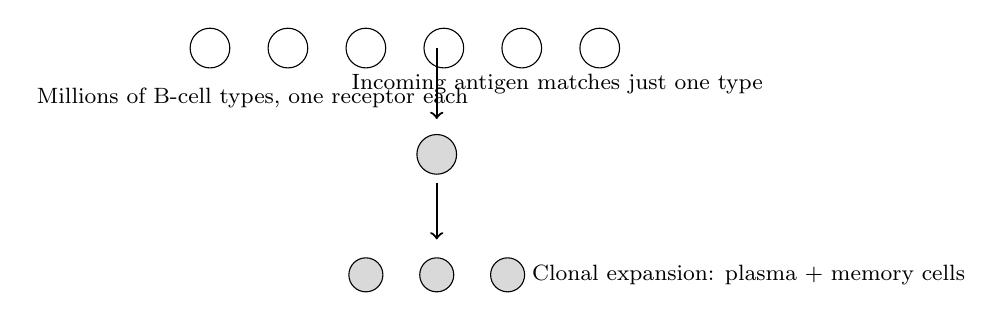
\begin{tikzpicture}[scale=0.9]
\foreach \i in {0,1,2,3,4,5} \draw[fill=white] (\i*1.1,2.2) circle (0.28);
\node at (0.6,1.5) {\footnotesize Millions of B-cell types, one receptor each};
\draw[->,thick] (3.2,2.2) -- (3.2,1.2);
\node at (4.9,1.7) {\footnotesize Incoming antigen matches just one type};
\draw[fill=gray!30] (3.2,0.7) circle (0.28);
\draw[->,thick] (3.2,0.3) -- (3.2,-0.5);
\draw[fill=gray!30] (2.2,-1.0) circle (0.24);
\draw[fill=gray!30] (3.2,-1.0) circle (0.24);
\draw[fill=gray!30] (4.2,-1.0) circle (0.24);
\node at (7.6,-1.0) {\footnotesize Clonal expansion: plasma $+$ memory cells};
\end{tikzpicture}
\end{center}
\vspace{-1em}
(A human schematic: circles show selection of one type from many, not actual cell appearances.)

Read those steps again. \textbf{Diversity, environmental selection, expansion of the selected} is natural selection's logic, formally explored in Chapter 76, now inside your body over days instead of hundreds of thousands of years. Immunity and evolution use the same algorithm. No prediction is required: the body prints enough lottery tickets, then waits for the winning numbers.

At a second encounter, memory cells skip the needle-in-a-haystack search and begin expanding within hours. Antibodies rise quickly and strongly, often suppressing the enemy before symptoms. That explains why chickenpox does not return: the virus is recognized and eliminated at the start, not frightened away.

\begin{zhengju}
Preexisting receptors selected by antigen seemed radical in the 1950s. The prevailing instruction theory pictured antibodies as modeling clay shaped around an incoming antigen template. It sounded economical: make only what is needed.

In 1957, the Australian immunologist F.~Burnet, Denmark's N.~Jerne, and others advanced the opposite view: each lymphocyte's antibody shape is randomly determined \textbf{before} antigen appears. Antigens judge rather than mold, selecting matching cells to multiply. Burnet predicted that each lymphocyte should make only one antibody specificity. Instruction theory gave no reason for that restriction: a cell should make whatever shape its current template required.

Decisive experiments followed a few years later. Researchers isolated single lymphocytes and cultured their descendants. Each clone recognized only one antigen and ignored others. Later molecular biology identified the DNA-level shuffling machinery that reassembles antibody genes during B-cell development, with DNA's information role explored from Chapter 67. Instruction theory was abandoned because its prediction failed and its rival's appeared. Burnet later received a Nobel Prize, but the point is not personal brilliance: \textbf{two explanations for antigen matching were separated by a different, testable prediction}.
\end{zhengju}

\section{Vaccines: A Safe Practice Exercise}

Clonal selection and memory explain vaccines in one sentence: \textbf{show the immune system the enemy's picture so it builds a file before the real encounter}.

A vaccine supplies antigens: perhaps a killed whole pathogen, a live one weakened until it cannot cause disease, a surface-protein fragment, or instructions for temporarily making that protein, as in mRNA vaccines and Chapter 68's transcription and translation. All \textbf{provide recognition targets, not the complete enemy}.

\textbf{Translator safety note:} The source simplifies vaccine categories: live attenuated vaccines contain whole, weakened organisms and can be unsuitable for some people, including those with certain immune deficiencies. Vaccines are medical products; suitability and dosing require professional guidance. See the \href{https://www.cdc.gov/pinkbook/hcp/table-of-contents/chapter-1-principles-of-vaccination.html}{CDC principles of vaccination}.

One frequent misconception needs particular care:

\textbf{A vaccine is not a medicine; it directly kills zero pathogens for you.} Antibiotics act directly on bacteria, with resistance discussed in Chapter 62. A vaccine directly kills \textbf{zero} pathogens. It triggers clonal selection: matching B cells expand and leave memory. Months later, \textbf{your own} antibodies and memory cells respond to the real virus. The injected material is gone; the trained immune system remains. Vaccination is a fire drill, not a hired fire brigade: the firefighters are still yours afterward.

Its effectiveness therefore depends on the recipient's immune system and varies individually. Protection and duration require \textbf{large population trials and long-term monitoring}, differing greatly among vaccines. This chapter explains evidence and mechanisms, not personal vaccination or treatment decisions. Those belong to clinicians and public-health agencies, whose assessments should guide decisions rather than a book.

The evidence story's first page goes back to 1796. The English physician E.~Jenner noticed milkmaids who had mild cowpox did not get deadly smallpox. He inoculated a boy with cowpox material; later smallpox exposure caused no illness. Jenner knew neither viruses nor antibodies, only an empirical rule: a related mild disease can prevent a severe one. Two centuries of data from vast populations repeatedly confirmed the principle, culminating in smallpox eradication in 1980, the first infectious disease deliberately eliminated by humanity. Clonal selection supplied the mechanism much later. \textbf{Effective practice can precede mechanistic theory}: knowing something works and knowing why are different kinds of evidence.

\section{Errors: Overreaction, Misdirection, and Missing Defenses}

Every recognition system errs. Three immune failures mark different stages of recognition, response, and memory, and this model's limits.

\begin{itemize}[itemsep=2pt]
\item \textbf{Allergy: overreacting to harmless targets.} Pollen, dust mites, and peanut proteins are harmless to most people, but some immune systems make IgE antibodies against them. Reexposure makes mast cells rapidly release histamine, sharply increasing vascular permeability and causing sneezing, runny nose, hives, or potentially fatal systemic anaphylaxis. The attack is real but misdirected. Genes and childhood exposures matter. The hygiene hypothesis suggests excessively clean childhood environments deprive immunity of training material, but \textbf{evidence is still accumulating}; it is not settled fact.
\item \textbf{Autoimmunity: attacking oneself.} Lymphocytes that recognize self antigens should be \textbf{deleted} during screening, but some escape. Activation of an escaped clone can attack tissues: islet cells in type 1 diabetes or joints in rheumatoid arthritis. Most such conditions can be controlled but are difficult to cure. Treatment often suppresses immunity at the cost of weakened defense, balancing harms.
\item \textbf{Immunodeficiency: a missing defense.} Some people are born lacking particular immune cells or antibodies. Alternatively, HIV attacks helper T cells, destroying command capacity and paralyzing the network. AIDS deaths result from successive infections by microbes ordinarily harmless.
\end{itemize}

\textbf{Translator safety note:} Suspected anaphylaxis is an emergency: use a prescribed adrenaline auto-injector as instructed and call emergency services immediately. See \href{https://www.nhs.uk/conditions/anaphylaxis/}{NHS anaphylaxis guidance}. The HIV passage describes severe immune failure, not an inevitable outcome: effective antiretroviral treatment supports long, healthy lives; see \href{https://hivinfo.nih.gov/understanding-hiv/fact-sheets/hiv-treatment-basics}{NIH HIV treatment information}.

Together these failures reveal that immunity aims not at maximum strength but at \textbf{precision}, balancing missed enemies against self-injury. Evolution selected not the greatest firepower but the lowest cost of mistakes.

\begin{wuqu}
``Stronger immunity is always better, so take supplements to boost it.'' Two errors: stronger reactions can mean allergy or autoimmunity, not health. And no supplement currently has high-quality evidence that it raises healthy people's immune function above normal. Most claims rest on cell or animal studies or uncontrolled testimonials. The real foundations are unremarkable: adequate sleep, balanced nutrition, regular exercise, and timely vaccination. Ask any immune-boosting claim whether its evidence is randomized controlled trials or advertising.
\end{wuqu}

\section{An Endless Arms Race}

The final piece is that enemies are not stationary targets.

Viruses and bacteria reproduce and vary. Some variants change antigen shape and escape existing antibodies; your immune pressure steers their evolution. Influenza changes its antigen coat yearly, requiring updated vaccines. Measles antigens scarcely change over decades, so one shot protects for decades. The difference lies not in vaccine technology but in \textbf{how quickly the enemy changes}.

\textbf{Translator safety note:} The one-shot measles analogy is not a vaccination schedule. CDC recommends two MMR doses for children; requirements for individuals depend on history and risk. Follow your clinician and current local guidance. See \href{https://www.cdc.gov/measles/vaccines/}{CDC measles vaccination information}.

Hosts evolve too. People with receptor variants resisting a pathogen may survive epidemics and leave more descendants. The sickle-cell gene's persistence in malarial regions is one trace of this contest, returning in Chapter 73. Pathogens and hosts have selected one another for hundreds of millions of years. Part X develops this arms-race logic fully.

\section{Back to the Small Wound}

Now fulfill the opening promise. First-day redness and heat follow innate patrols detecting bacteria entering a paper cut. Their signals widen vessels and recruit help. Redness, swelling, warmth, and pain are not signs of worsening but \textbf{the battlefield itself}. Phagocytes then remove bacteria and dead tissue; if viruses are involved, adaptive clonal selection quietly proceeds in lymphoid organs. Afterward, epidermal cells close the gap and the scab falls. If a vaccine-targeted pathogen entered, memory cells could handle it unnoticed. Your record matters because of trained cells in lymph nodes and bone marrow, not because the recorded fluid remains.

\textbf{Translator safety note:} Redness and swelling can also signal a worsening infection. The source's battlefield analogy must not override its earlier warning: spreading redness, increasing pain, or fever needs prompt medical advice. See \href{https://www.nhs.uk/conditions/cuts-and-grazes/}{NHS wound guidance}.

At a vaccine's tiny injection site, a miniature exercise similarly produces a little redness and a batch of memory.

\section{Next Chapter's Puzzle}

You may have noticed a major gap: your gut contains \textbf{trillions of bacteria} weighing more than a kilogram. Under an attack-all-nonself rule, every one should be destroyed. Yet the body tolerates and depends on them. How does immunity overlook some nonself, and how can we coexist with microbes? You are not simply an individual but a walking ecosystem. Next chapter, meet your tenants.

\begin{tiaozhan}
How is antibody diversity shuffled? Variable-region genes contain segment libraries: about $40$ V, $25$ D, and $6$ J segments for the heavy chain, with counts varying by definition. A maturing B cell picks one from each, giving $40\times 25\times 6=6000$ heavy chains. Independently assembled light chains add about $300$ combinations. Pairing them gives $6000\times 300\approx 2\times 10^{6}$. Random nucleotide insertion and deletion at joins adds unbounded randomness, raising diversity above $10^{11}$. Activated B cells further accelerate mutation in variable regions and select better variants through somatic hypermutation, ultimately recognizing tens of quadrillions of shapes. Diversity comes from \textbf{controlled randomness}, not foreknowledge.
\end{tiaozhan}

\section*{Practice}

\begin{sikaoti}
\item Draw an invasion information-flow map from a skin breach, showing where innate phagocytes and adaptive B and T cells intervene and exchange alarm or confirmation signals. Note that arrows indicate information or material transfer, not cells literally queuing.
\item Use clonal selection's three steps to explain why a first vaccine may need one or two weeks for sufficient antibodies, whereas a real encounter six months later produces many within one or two days. Mark which stage memory cells change.
\item Refute: vaccine antigen triggers immunity, so a vaccine is itself a pathogen and receiving it means becoming ill. Distinguish recognition targets from complete enemies and compare attenuated, inactivated, and protein-fragment vaccines.
\item Allergy and autoimmunity are often called excessive immunity. Identify what actually fails in each and explain why boosting immunity is not a good response.
\item Research one pathogen with nearly stable antigens and long-lasting single-shot vaccine protection, and another with rapidly varying antigens requiring vaccine updates. Explain using variation as diversity and immunity as selection pressure. Which evolutionary logic learned before Chapter 10 has the same structure?
\item With roughly $2\times 10^{20}$ antibodies in the body, suppose $10^{8}$ plasma cells derived from memory B cells each secrete $2000$ antibodies per second. How many are produced daily? What does comparison with the existing stock tell you?
\end{sikaoti}
